\documentclass[11pt]{article}
\usepackage[margin=1in]{geometry}
\usepackage{amsmath}
\usepackage{amssymb}
\usepackage{tikz}
\usetikzlibrary{arrows.meta, positioning, shapes.geometric}

\title{Reinforcement Learning for Maximum-Flow Interdiction}
\author{}
\date{}

\begin{document}
\maketitle

\section{Problem}
The goal is to remove at most \(B=2\) edges from a directed, capacitated
network to minimize the remaining maximum flow from source \(s\) to sink \(t\).
The sample network contains three edge-disjoint routes:

\begin{center}
\begin{tabular}{c|c|c}
Edge index & Directed edge & Capacity \\
\hline
0 & \(s \to a\) & 2 \\
1 & \(a \to t\) & 2 \\
2 & \(s \to b\) & 3 \\
3 & \(b \to t\) & 3 \\
4 & \(s \to c\) & 1 \\
5 & \(c \to t\) & 1
\end{tabular}
\end{center}

Before interdiction, the maximum flow is \(2+3+1=6\).

\section{Mathematical Formulation}
Let \(G=(V,E)\) be the directed network, \(s\) the source, \(t\) the sink,
\(c_e>0\) the capacity of edge \(e\), and \(B\) the interdiction budget.
For each edge, \(z_e=1\) means that it is removed, while \(x_e\) is its
flow. The interdiction problem is the following leader--follower optimization:
\[
\begin{aligned}
\min_{z\in\{0,1\}^{|E|}}\quad
    & \max_{x\geq 0,\,q\geq 0} q \\
\text{subject to}\quad
    & \sum_{e\in\delta^+(v)}x_e-\sum_{e\in\delta^-(v)}x_e=0,
      && v\in V\setminus\{s,t\},\\
    & \sum_{e\in\delta^+(s)}x_e-\sum_{e\in\delta^-(s)}x_e=q,\\
    & \sum_{e\in\delta^-(t)}x_e-\sum_{e\in\delta^+(t)}x_e=q,\\
    & 0\leq x_e\leq c_e(1-z_e),
      && e\in E,\\
    & \sum_{e\in E} z_e\leq B.
\end{aligned}
\]
Here, \(\delta^+(v)\) and \(\delta^-(v)\) are the outgoing and incoming
edges of node \(v\). The inner maximization computes the maximum flow after
the interdiction decisions; the outer minimization selects the edges to
remove. Since removing extra edges cannot increase maximum flow, the
at-most-\(B\) budget is consistent with the code's use of the full budget
when at least \(B\) edges exist.

\section{Method}
The Q-learning state at step \(k\) is the set \(S_k\subseteq E\) of already
removed edges. Its legal actions are \(e\in E\setminus S_k\); taking action
\(e\) gives next state \(S_{k+1}=S_k\cup\{e\}\). The reward is the reduction
in maximum flow:
\[
  r(S_k,e) = F(S_k)-F(S_k\cup\{e\}),
\]
where \(F(S)\) denotes the maximum flow after removing edges \(S\). The
episode ends when \(B\) edges have been removed or no legal edges remain.
The undiscounted sum of rewards telescopes to the initial flow minus the
final flow; therefore, maximizing reward minimizes the final flow.

\subsection{Agent and Evaluation Process}
\begin{center}
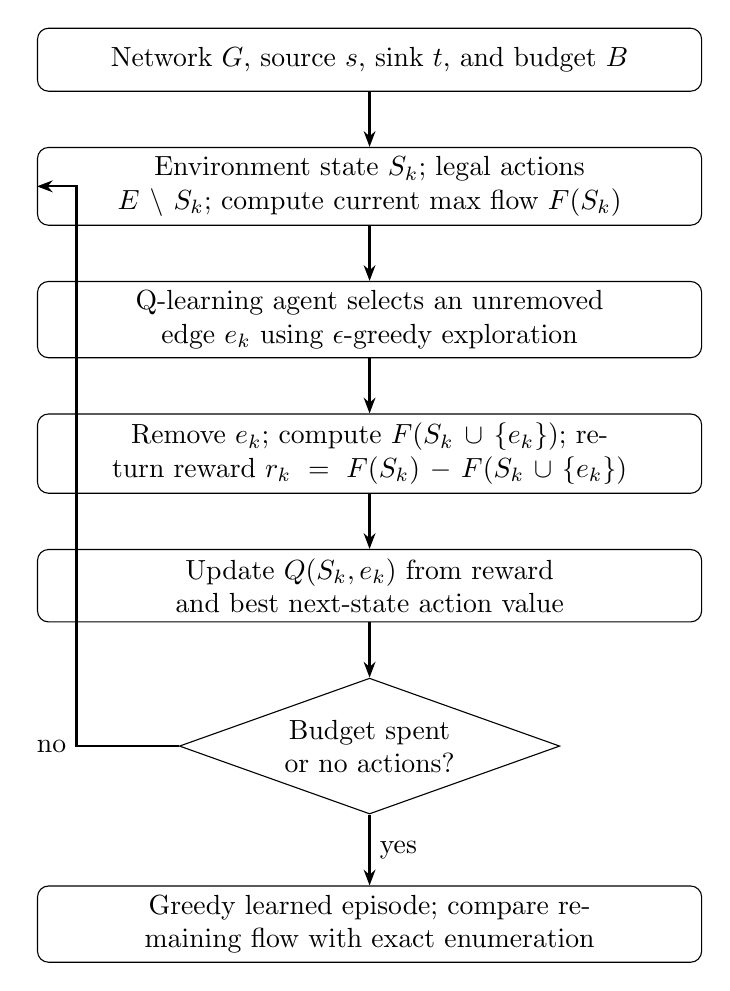
\begin{tikzpicture}[
  node distance=7mm and 12mm,
  box/.style={draw, rounded corners, align=center, text width=8.2cm,
              minimum height=8mm},
  decision/.style={draw, diamond, aspect=2.8, align=center,
                   text width=2.7cm, inner sep=1pt},
  arrow/.style={-{Stealth[length=2mm]}, thick}
]
\node[box] (input) {Network \(G\), source \(s\), sink \(t\), and budget \(B\)};
\node[box, below=of input] (state) {Environment state \(S_k\); legal actions
  \(E\setminus S_k\); compute current max flow \(F(S_k)\)};
\node[box, below=of state] (agent) {Q-learning agent selects an unremoved edge
  \(e_k\) using \(\epsilon\)-greedy exploration};
\node[box, below=of agent] (transition) {Remove \(e_k\); compute
  \(F(S_k\cup\{e_k\})\); return reward
  \(r_k=F(S_k)-F(S_k\cup\{e_k\})\)};
\node[box, below=of transition] (update) {Update \(Q(S_k,e_k)\) from reward
  and best next-state action value};
\node[decision, below=of update] (done) {Budget spent or no actions?};
\node[box, below=of done, yshift=-2mm] (compare) {Greedy learned episode;
  compare remaining flow with exact enumeration};
\draw[arrow] (input) -- (state);
\draw[arrow] (state) -- (agent);
\draw[arrow] (agent) -- (transition);
\draw[arrow] (transition) -- (update);
\draw[arrow] (update) -- (done);
\draw[arrow] (done) -- node[right, align=left] {yes} (compare);
\draw[arrow] (done.west) -- ++(-1.3,0) node[left] {no}
  |- (state.west);
\end{tikzpicture}
\end{center}

\subsection{Algorithms}
Maximum flow is calculated using Edmonds--Karp: repeatedly find a
shortest-in-edges augmenting path by breadth-first search in the residual
network, augment by the path's bottleneck capacity, and stop when no such
path exists.

\paragraph{Edmonds--Karp pseudocode}
\begin{verbatim}
Initialize residual capacities from all non-removed edges
total_flow = 0
While BFS finds a residual path from source to sink:
    delta = minimum residual capacity on that path
    update forward and reverse residual capacities by delta
    total_flow = total_flow + delta
Return total_flow
\end{verbatim}

The Q-learning update in the implementation uses learning rate \(\alpha\)
and discount factor \(\gamma=1\):
\[
Q(S_k,e_k)\leftarrow Q(S_k,e_k)+
\alpha\left[r_k+\gamma\max_{e'\in E\setminus S_{k+1}}
Q(S_{k+1},e')-Q(S_k,e_k)\right].
\]
The maximum next-action value is defined as zero at a terminal state. The
behavior policy explores with probability \(\epsilon\), otherwise choosing
among actions with the greatest current Q-value. Epsilon decreases linearly
from its initial to final value over training.

\paragraph{Training pseudocode}
\begin{verbatim}
Initialize Q(S,e) = 0 for each state-action pair
For each episode:
    S = empty set
    While |S| < min(B, |E|):
        choose e from E \ S using epsilon-greedy policy
        S_next = S union {e}
        r = F(S) - F(S_next)
        update Q(S,e) toward r + max_a Q(S_next,a)
            (use 0 for the next-action value at a terminal state)
        S = S_next
Return an episode by greedily selecting the best Q-valued legal action
\end{verbatim}

The exact baseline enumerates every subset of edges of size at most \(B\),
computes its remaining maximum flow, and returns a subset with minimum flow.
It is practical for this small example, but its number of candidates grows
combinatorially.

\paragraph{Exact enumeration pseudocode}
\begin{verbatim}
best_flow = F(empty set)
best_set = empty set
For each edge subset S with |S| <= min(B, |E|):
    flow = Edmonds-Karp after removing S
    If flow < best_flow:
        best_flow = flow
        best_set = S
Return best_set, best_flow
\end{verbatim}

The run used 20,000 episodes, learning rate \(\alpha=0.2\), a linearly
decreasing exploration rate from 1.0 to 0.05, and random seed 7. Maximum flow
was computed with Edmonds--Karp. As an exact baseline, all removal sets of
size at most two were enumerated; for six edges, this is
\[
  \binom{6}{0}+\binom{6}{1}+\binom{6}{2}=22
\]
candidate sets.

\section{Results}
Both Q-learning and exact enumeration selected edge indices \(0\) and \(2\),
removing \(s \to a\) and \(s \to b\). Only the route through \(c\) remains, so
the maximum flow is 1.

\begin{center}
\begin{tabular}{l|r}
Measure & Result \\
\hline
Initial maximum flow & 6 \\
Interdiction budget & 2 edges \\
Q-learning remaining flow & 1 \\
Exact optimum remaining flow & 1 \\
Optimality gap & 0
\end{tabular}
\end{center}

On this sample, the learned result matches the exact optimum. This does not
establish optimality on larger networks; exact enumeration grows
combinatorially, and tabular Q-learning performance depends on the network,
training duration, and random seed.

\section{Reproduction}
From the project directory, run:
\begin{verbatim}
python max_flow_interdiction.py
python -m unittest -v test_max_flow_interdiction.py
\end{verbatim}
\begin{verbatim}
Source: max_flow_interdiction.py
Tests:  test_max_flow_interdiction.py
\end{verbatim}

\end{document}
